
\documentclass[a4paper, 12pt, onecolumn, oneside]{report}

\usepackage{geometry} 
\geometry{a4paper} 
\usepackage{graphicx} 
\usepackage{float}
\usepackage{wrapfig} 
\usepackage{lipsum} 
\usepackage  [utf8] {inputenc}
\usepackage  [portuguese] {babel}
\linespread{1.2}
%\setlength\parindent{0pt} 
\graphicspath{{./Imagens/}} 
\usepackage{graphicx}
\begin{document}
\begin{titlepage}

\newcommand{\HRule}{\rule{\linewidth}{0.4mm}} % 

\center 


\begin{figure}[H] 
\center{
\includegraphics[width=1.0\linewidth]{UA1}}
\end{figure}


\textsc{\ Departamento de Electrónica, Telecomunicações e Informática
 }\\[0.9cm] 

{\raggedright \textbf{Curso:} [8240] Mestrado Integrado em Eng. de Computadores e Telemática

\textbf{Disciplina:} [47137] Introdução à Eng. de Computadores e Telemática

\textbf{Ano lectivo:} 2012/2013 \\[1cm] 

}


\HRule \\[0.1cm]
{ \huge \bfseries Relatório da Aula Prática 9 \\
[0.4cm]  
Programação do Robô \\ [0.4cm] DETI PIC }\\[0.4cm] 
\HRule \\[1cm]


\begin{minipage}{0.4\textwidth} 
\begin{flushleft} \large
\emph{Autores:}\\
{[68535] Bruno \textsc{Silva}} \\
{[68799] Rui \textsc{Oliveira} } 


\emph{Turma/Grupo:}\\
T5B / Prática 3\\

\end{flushleft}
\end{minipage}
~
\begin{minipage}{0.4\textwidth}
\begin{flushright} \large
\emph{Docentes:} \\
André \textsc{Zúquete} \\
João \textsc{Barraca} \\
\emph{Data:} \\
\today 
\end{flushright}
\end{minipage}\\[2cm]



\vfill 

\end{titlepage}



\vspace*{\fill}



\textbf{Resumo:}


\begin{flushleft}

 Pretende-se através deste relatório expor sob forma escrita, o nosso desempenho e objetivos alcançados na aula de Introdução à Engenharia de Computadores e Telemática sobre a programação do robô DETI PIC, desenvolvido pelo Departamento de Eletrónica, Telecomunicações e Informática da Universidade de Aveiro.

\end{flushleft}


\vspace*{\fill}

\newpage




\newpage

\renewcommand*\contentsname{Índice}

\tableofcontents 


\newpage
 
\section{Introdução} 


Como sabemos, um robô é um dispositivo, ou conjunto de dispositivos, eletromecânicos ou biomecânicos capazes de realizar uma determinada funcionalidade de forma independente, para isso terá de ser pré-programado, ou então controlado por um ser humano. Primordialmente os robôs foram programados para desenvolver trabalhos de baixa complexidade, como por exemplo, deslocarem-se sobre superfícies planas, interagir com obstáculos, entre outros. Atualmente, os robôs realizam tarefas muito completas, e em muitos dos casos substituindo o trabalho humano. Embora, nem sempre se tira partido de todas as capacidades do robô.

Neste relatório pretendemos demonstrar o nosso desempenho na programação do robô DETI PIC, desenvolvido pelo Departamento de Eletrónica, Telecomunicações e Informática da Universidade de Aveiro. Mais à frente iremos mostrar as principais características do robô, e alguns dos equipamentos e materiais que utilizámos para conseguir concretizar esta actividade. Para a programação de robô utilizando um software, também este desenvolvido pelo DETI, chamado \emph{DETInchanting} criado a partir de linguagem JAVA e C++ e adaptado do \emph{Enchanting}, desenvolvido para robôs da LEGO\footnote{Empresa conceituada no fabrico de brinquedos, e atualmente no desenvolvimento de robôs. }. Neste caso, necessitámos de ter conhecimentos básicos de programação em JAVA, para conseguir testar as capacidades do robô, através da implementação blocos que permitem executar operações do tipo: \emph{if}... \emph{else}...; \emph{forever}... ; \emph{repeat until}... ; entre outros. 

Ambicionamos com estes testes ao robô, neste relatório, explorar essencialmente os sensores de brilho, embora também iremos utilizar os sensores de distância. Através dos sensores de brilho iremos programar o robô de modo que este siga uma linha preta em diferentes perspectivas. Mais à frente neste relatório iremos explicar detalhadamente quais serão estas perspectivas. 







\newpage
\section{Descrição do problema}

Pretendemos através deste relatório dar resposta, programando e observando o comportamento do robô DETI PIC de modo a solucionar os seguintes problemas apresentados: 

\begin{itemize}
  \item \textbf{PROBLEMA 1} - Programar o robo de forma a ele seguir uma linha cuja largura é inferior à distância entre os dois sensores em torno do central (\emph{left} e \emph{right}, no \emph{DETInchanting}). Nesta linha poderá aparecer um entrocamento que deverá ser ignorado. No final da linha o robô deverá parar, de acordo com a figura seguinte. 
  
  
\begin{figure}[H] 
\center{
\includegraphics[width=0.5\linewidth]{f1}}
\caption{Esquema do problema 1.}
\label{fig:speciation}
\end{figure}
  
\end{itemize}

\begin{itemize}
  \item \textbf{PROBLEMA 2} - Alterar o primeiro programa de modo a que o robô pare durante um segundo, com os 4 leds acesos, quando encontrar o entrocamento. Após essa paragem deverá apagar os leds, retomando o seu movimento e não parar novamente no mesmo entroncamente. 
\end{itemize}


\newpage
\begin{itemize}
  \item \textbf{PROBLEMA 3} - Alterar o programa do Problema 1 de modo a que o robô volte para trás no final da linha. (Ver Figura 2)
\end{itemize}



  \begin{figure}[H] 
\center{
\includegraphics[width=0.5\linewidth]{f2}}
\caption{Esquema do problema 3.}
\label{fig:speciation}
\end{figure}



\begin{itemize}
  \item \textbf{PROBLEMA 4} - Alterar o programa anterior para que o robô siga a linha à direita sempre que encontra um entroncamento. (Ver Figura 3)
\end{itemize}


\begin{figure}[H] 
\center{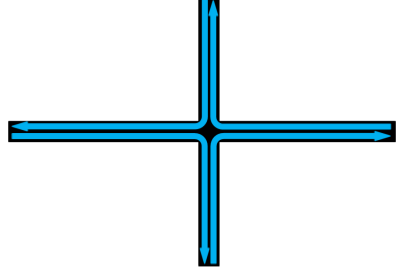
\includegraphics[width=0.5\linewidth]{f3}}
\caption{Esquema do problema 4.}
\label{fig:speciation}
\end{figure}

\newpage

\begin{itemize}
  \item \textbf{PROBLEMA 5} - Alterar um dos quantro problemas acima mencionados, mas agora prevendo o facto de poder existir uma parede a interromper a linha. Neste caso o robô deverá abandonar a linha, seguir a parede e voltar a seguir a linha, abandonando a parede, quando reencontrar a primeira. (Ver Figura 4)
\end{itemize}


\begin{figure}[H] 
\center{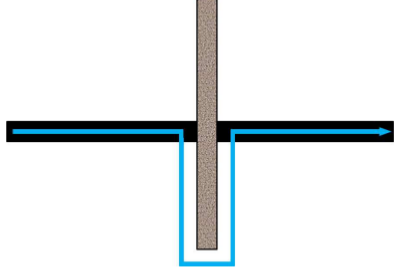
\includegraphics[width=0.5\linewidth]{f4}}
\caption{Esquema do problema 5.}
\label{fig:speciation}
\end{figure}



Para além dos cinco problemas acima descritos, pretendemos também adquirir alguns dos conhecimentos introdutórios do funcionamento e programação da robótica utilizando para isso o \emph{DETInchanting}, programa este que iremos abordar mais à frente. Dado que nos foi imposto a realização deste relatório utilizando a linguagem tipo \LaTeX, pretendemos também desenvolver as nossas competências a nível desta linguagem, alargando assim os nossos conhecimentos já adquiridos em aulas anteriores.


\newpage
\section{Aparelhagem e equipamento}



\subsection{Robô DETI PIC}

A nossa base de trabalho é o robô DETI PIC. Este robô é constituído por dois motores DC\footnote{Corrente contínua} sem realimentação, três sensores de distância frontais cobrindo um ângulo de aproximadamente 45 graus para cada lado do robô, cinco sensores de brilho na parte inferior do robô e quatro led's na parte superior. O robô dispõe ainda de dois botões, um interruptor e uma porta USB. Todo este robô foi desenvolvido de forma prática e intuitiva à introdução à programação deste tipo de máquinas. 
Para fazer o upload entre o robô e o computador utilizá-mos um cabo USB\footnote{Universal Serial Bus} 2.0.



\begin{figure}[H] 
\center{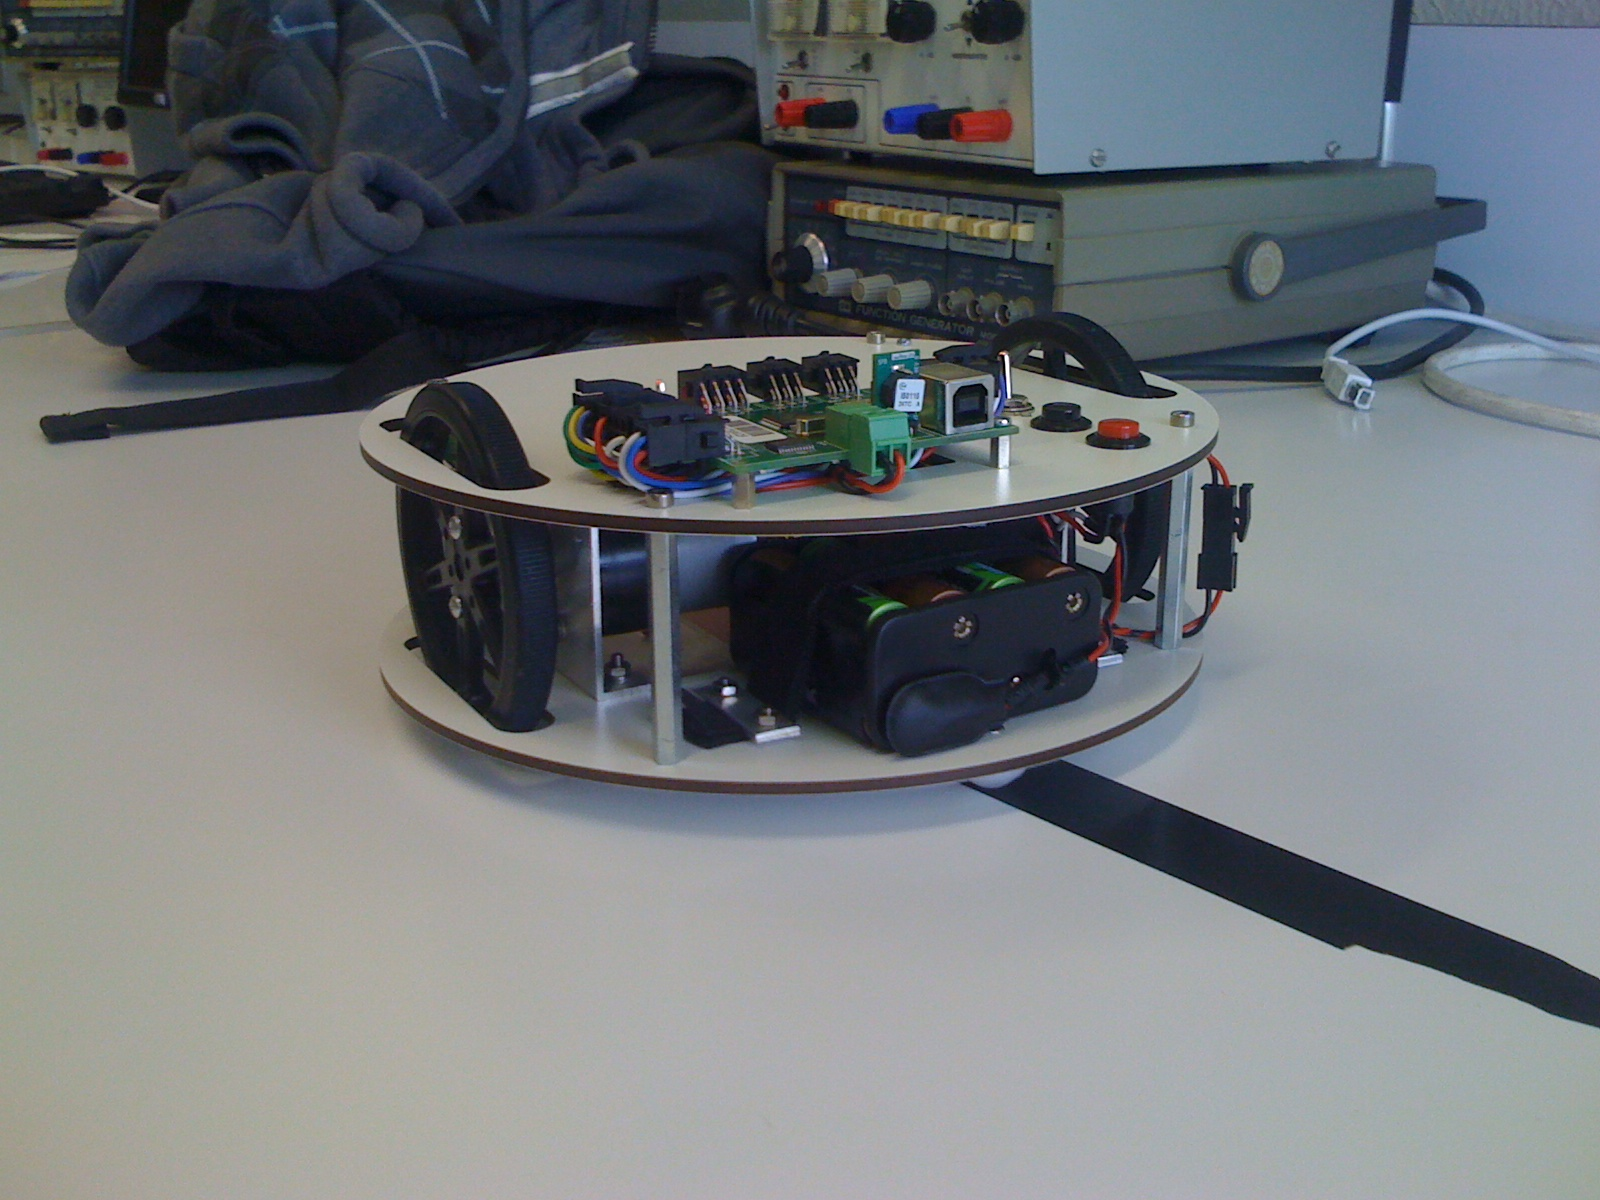
\includegraphics[width=0.5\linewidth]{robo2}}
\caption{Robô DETI PIC}
\label{fig:speciation}
\end{figure}


\subsection{Software DETInchanting}

O programa usado para a programação de instruções a dar ao robô neste trabalho foi o \emph{DETInchanting}, uma adaptação do original \emph{Enchanting} usado para programar robôs da LEGO. Este interface foi desenvolvido na Universidade de Aveiro com a intenção de facilitar a programação dos robôs utilizando um interface gráfico que se baseava em encaixes de blocos de código JAVA, na Figura 2 está representada o ambiente de trabalho deste programa. Este sofware usa um paradigma gráfico do tipo Scratch\footnote{São interfaces gráficos que permitem que programas sejam criado através da sobreposição de blocos, tendo na sua base linguagens de programação.}.



\begin{figure}[H] 
\center{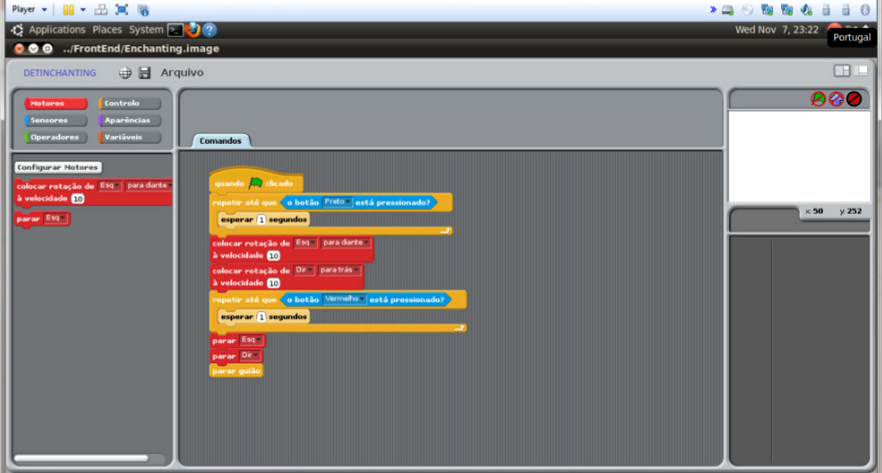
\includegraphics[width=0.9\linewidth]{ambiente}}
\caption{Ambiente do \emph{DETInchanting.}}
\label{fig:speciation}
\end{figure}




\subsection{Materiais utilizados}

O nosso ambiente de trabalho foi a bancada dos laboratórios do DETI o que não nos dava muito espaço para manobrar o robô. Nestas condições usamos duas linhas de cor preta cruzadas entre si, para realização dos problemas propostos. Para a realização do Problema 5 utilizámos uma parede em K-Line.  


 \newpage
 
\section{Procedimento}

\subsection{Problema 1}

Neste problema tal como nos restantes, começámos por introduzir um ciclo \emph{repeat until}, que nos permite ao pressionar no botão red, que o programa seja executado.  

Seguidamente, num ciclo repetitivo \emph{forever}, introduzimos uma condição “Is dark from LEFT or RIGTH or CENTER sensor?”, esta opção irá possibilitar que o robô siga a linha escura, e caso se desvie(ou seja, se o sensor de brilho deixar de observar a cor preta) irá ser corrigida através da implementação de um bloco condicional. Por exemplo se a condição “Is dark from LEFT sensor?” se verificar, então o motor da roda esquerda irá parar e apenas o da direita se irá movimentar, de modo que a condição anteriormente descrita se deixe de verificar. O mesmo acontece no caso RIGTH, mas neste caso o movimento das rodas será trocado. Na situação “Is dark from CENTER sensor?” ambos os motores irão funcionar, ao mesmo tempo. Neste caso tivemos particular atenção à velocidade de cada roda, devido à folga que existe numa delas, por isso utilizámos a velocidade 60 e 55 para o motor esquerdo e direito, respectivamente. 

Num outro ciclo \emph{if} , caso se verifique a condição “Is dark from LEFT and RIGTH and CENTER and FAR LEFT and FAR RIGTH sensor?”, o dois motores irão deslocar-se em frente à mesma velocidade que anteriormente se movimentavam. Esta circunstância ocorre quando o robô encontra o entroncamento. Esta funcionalidade permite ao robô, quando os seus sensores de brilho mais laterais encontrarem o cruzamento, ou seja quando a condição anteriormente descrita se verificar, o robô irá ignorar o cruzamento, e seguirá em frente.  

No final do problema, no \emph{else} das condições acima descritas o robô irá parar (\emph{stop all}), ou seja quando deixar de detetar qualquer linha preta nos seus sensores centrais, o robô irá por completo o seu percurso.


\newpage

\subsection{Problema 2}

Para a resolução deste problema começámos por introduzir uma estrutura de repetição \emph{repeat until} sempre que o sensor \emph{far right} e o sensor \emph{far left} detestassem escuro. Caso isso acontecesse, quando o sensor \emph{center} detetasse a mesma condição, então o motor esquerdo e direita irão mover-se os dois, caso o sensor a detetar fosse o "\emph{right}" então, a roda direita irá parar e apenas a do lado esquerdo irá movimentar-se, analogamente o mesmo acontece caso seja o sensor \emph{left} a detetar presença da cor negra. A organização acima descrita permite que o robô corrija a sua posição em relação à linha, o mesmo aconteceu no programa 1.

Numa outra estrutura de estado, do tipo \emph{if}, introduzimos uma condição que permite ao robô, ao encontrar o entroncamento, ou seja, caso o sensor \emph{far rigth} e \emph{far left} (estes localizados nas extremidade do robô) detete linhas escuras, então o robô irá parar (velocidade de ambos os motores será zero), e posteriormente irá ligar os seus led’s durante 1 segundo. 

De seguida, obtivemos um ciclo \emph{forever} que permite ao robô, quando este chegar ao fim da linha que volte para trás. Para conseguir este sucedido procedemos da mesma forma tal como quando queríamos que o robô corrigir a linha no início do programa. Para finalizar o nosso projeto, voltamos a introduzir uma nova estrutura \emph{if} que nos permite, quando o robô passar novamente pelo cruzamento irá ignorá-lo e seguirá em frente, ou seja quando “Is dark from LEFT and RIGTH and CENTER and  LEFT and sensor? = false”, então o motor direito e da esquerda irá seguir em frente.

Tal como no programa anterior, tivemos especial atenção à velocidade que atribuímos ao motor esquerdo e direito, pois devido à existência de uma pequena folga o robô desviava-se intencionalmente.

\newpage

\subsection{Problema 3}

Neste programa começamos com um ciclo \textit{forever} que vai acompanhar o resto do programa até ao fim contendo no seu interior uma sequência de 5 \textit{if's} acompanhados por os respectivos \textit{elses's} encadeados de forma a tornar o processo de processamento do código mais eficiente pelo robô, tentando com isto tornar o robô mais reactivo às diferente situações que tinha de enfrentar. Os \textit{if's} estão delineados de forma a que o robô avalie as situações da melhor forma tentando neste caso ignorar o cruzamento a meio do trajecto, e no final da linha "dar a a volta" repetindo sempre este ciclo. O primeiro \textit{if} do nosso código avalia se o robô esta a andar em cima da linha preta de forma correcta, enquanto que o segundo e terceiro fazem as devidas correcções para a direita e esquerda respectivamente. O \textit{if} seguinte trata de ignorar o cruzamento enquanto que o ultimo faz com que o robô "dê a volta" quando deixar de encontrar a linha preta.

Por ultimo adicionamos um \emph{if} que de certa forma era um pouco opcional que fazia o código parar assim que pressionarmos o botão preto.


\subsection{Problema 4}

Este programa foi o mais complexo que resolvemos. Para o solucionar dentro do ciclo \textit{forever} o programa encontra um \textit{if} que verifica se o robô se encontra em cima da linha ou não, caso se encontre vai haver outro \textit{if} que vai avaliar o caso de este se encontrar num cruzamento e começa o processo de virar a direita através de dois \textit{repeat until} o primeiro fazendo virar até a linha passar o sensor direito \textit{(right)} e o segundo até a linha encontrar o sensor \textit{(center)} central do robô. Como faria sentido o \textit{else} de encontrar o cruzamento quando se encontra na linha é de andar em frente seguindo a linha até o cenário que o robô encontre mude e ele tenha de agir de forma diferente. Com esta mudança de cenário entra o \textit{else} do primeiro \textit{if} que neste caso é quando o robô não encontra linha preta no sensor central \textit{(center)} e com isto vai tomar uma de e decisões, corrigir a posição à esquerda, à direita ou então "dar a volta". Como nos outros programas é acrescentado um ultimo \textit{if} para parar o programa a quando o botão preto é pressionado.






 \newpage
\section{Resultados}

\subsection{Problema 1}

Através da implementação, criação e posterior uploud do programa apresentado na Figura 7, conseguimos obdecer ao enunciado do Problema 1.

\begin{figure}[H]
\center{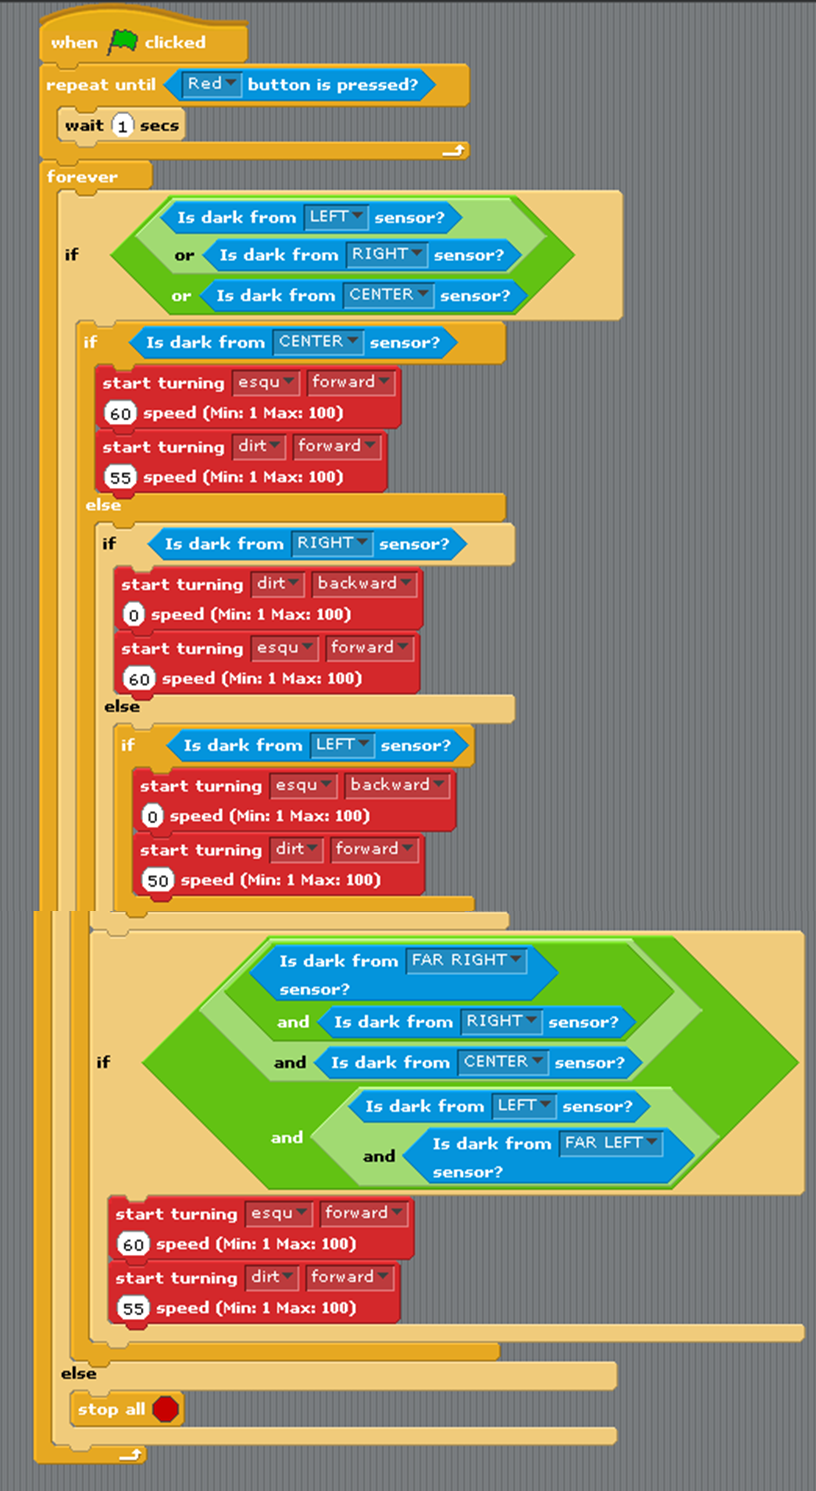
\includegraphics[width=0.6\linewidth]{ex1}}
\caption{Resolução do problema 1 utilizando o sofware DETInchanting.}
\label{fig:speciation}
\end{figure}

\subsection{Problema 2}

Através da implementação, criação e posterior uploud do programa apresentado na Figura 8, conseguimos obdecer ao enunciado do Problema 2.

\begin{figure}[H]
\center{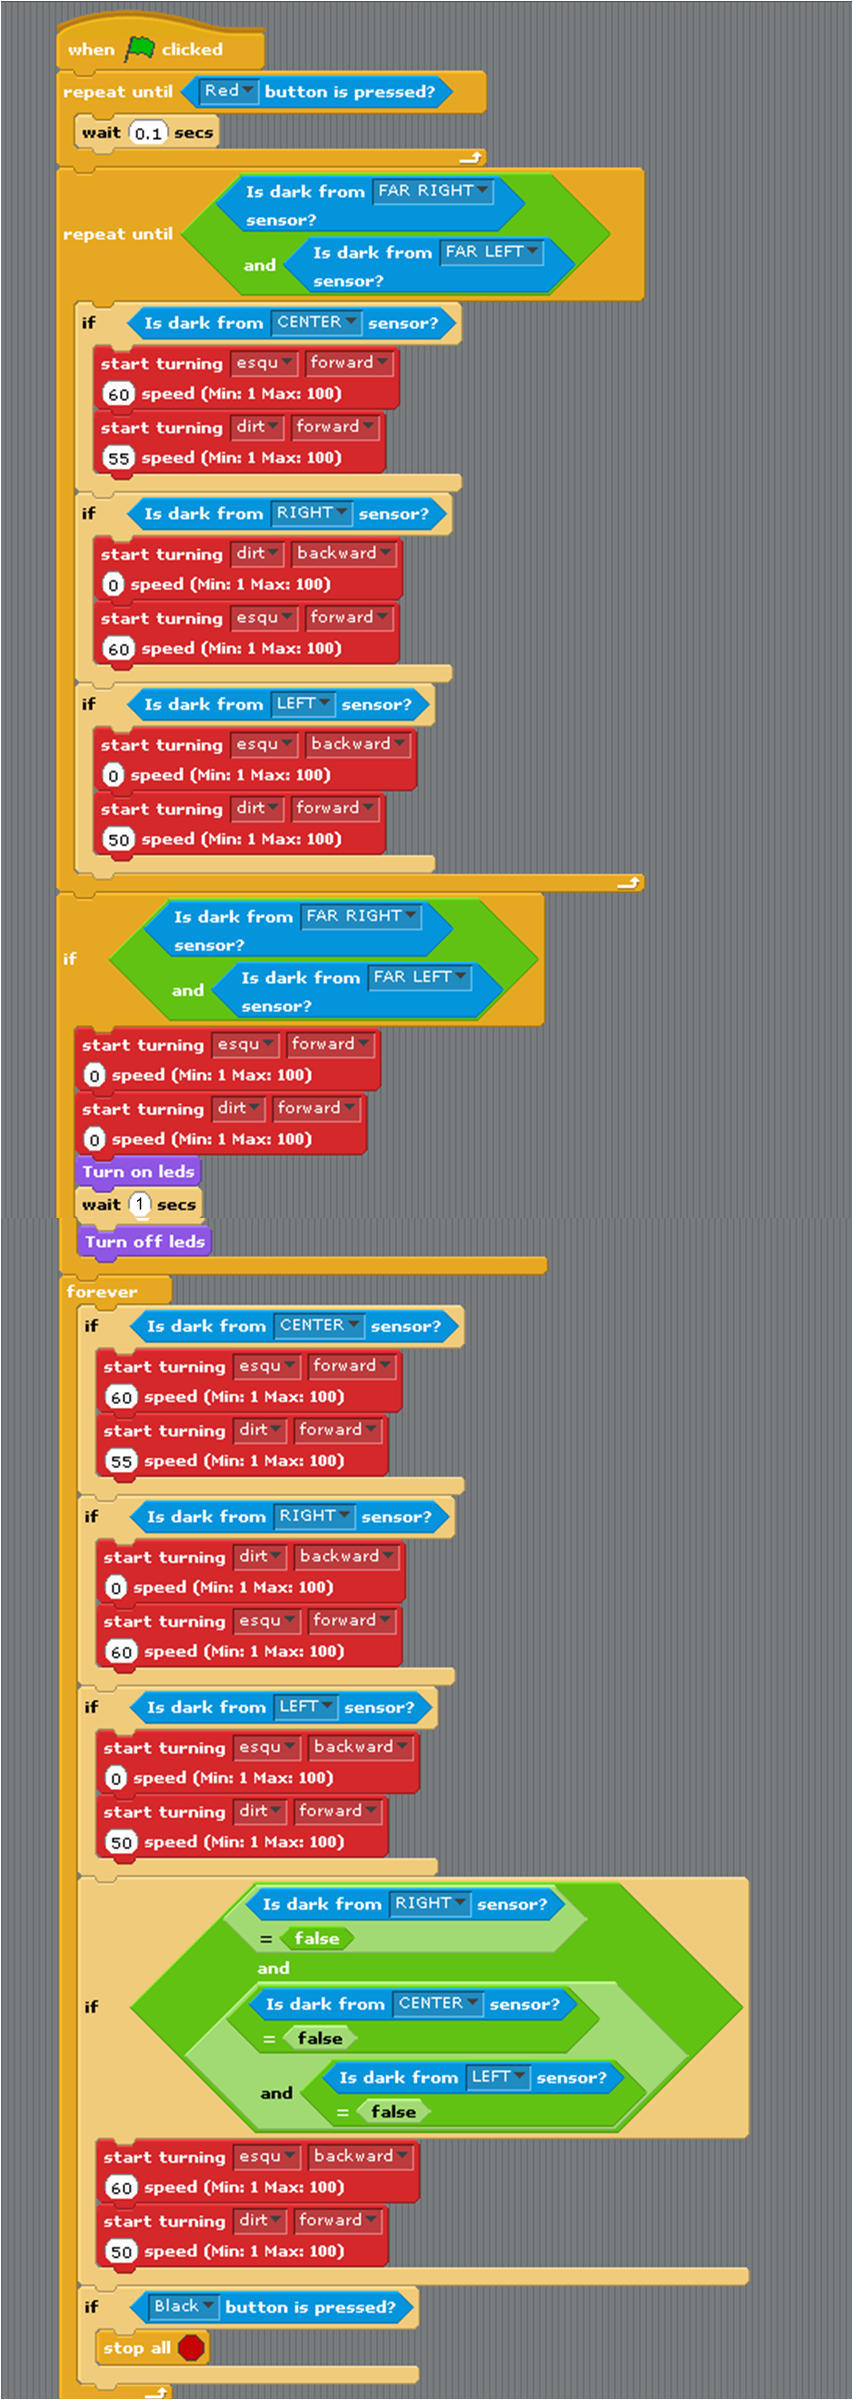
\includegraphics[width=0.4\linewidth]{ex2}}
\caption{Resolução do problema 2 utilizando o sofware DETInchanting.}
\label{fig:speciation}
\end{figure}

\subsection{Problema 3}

Através da implementação, criação e posterior uploud do programa apresentado na Figura 9, conseguimos obdecer ao enunciado do Problema 3.

\begin{figure}[H]
\center{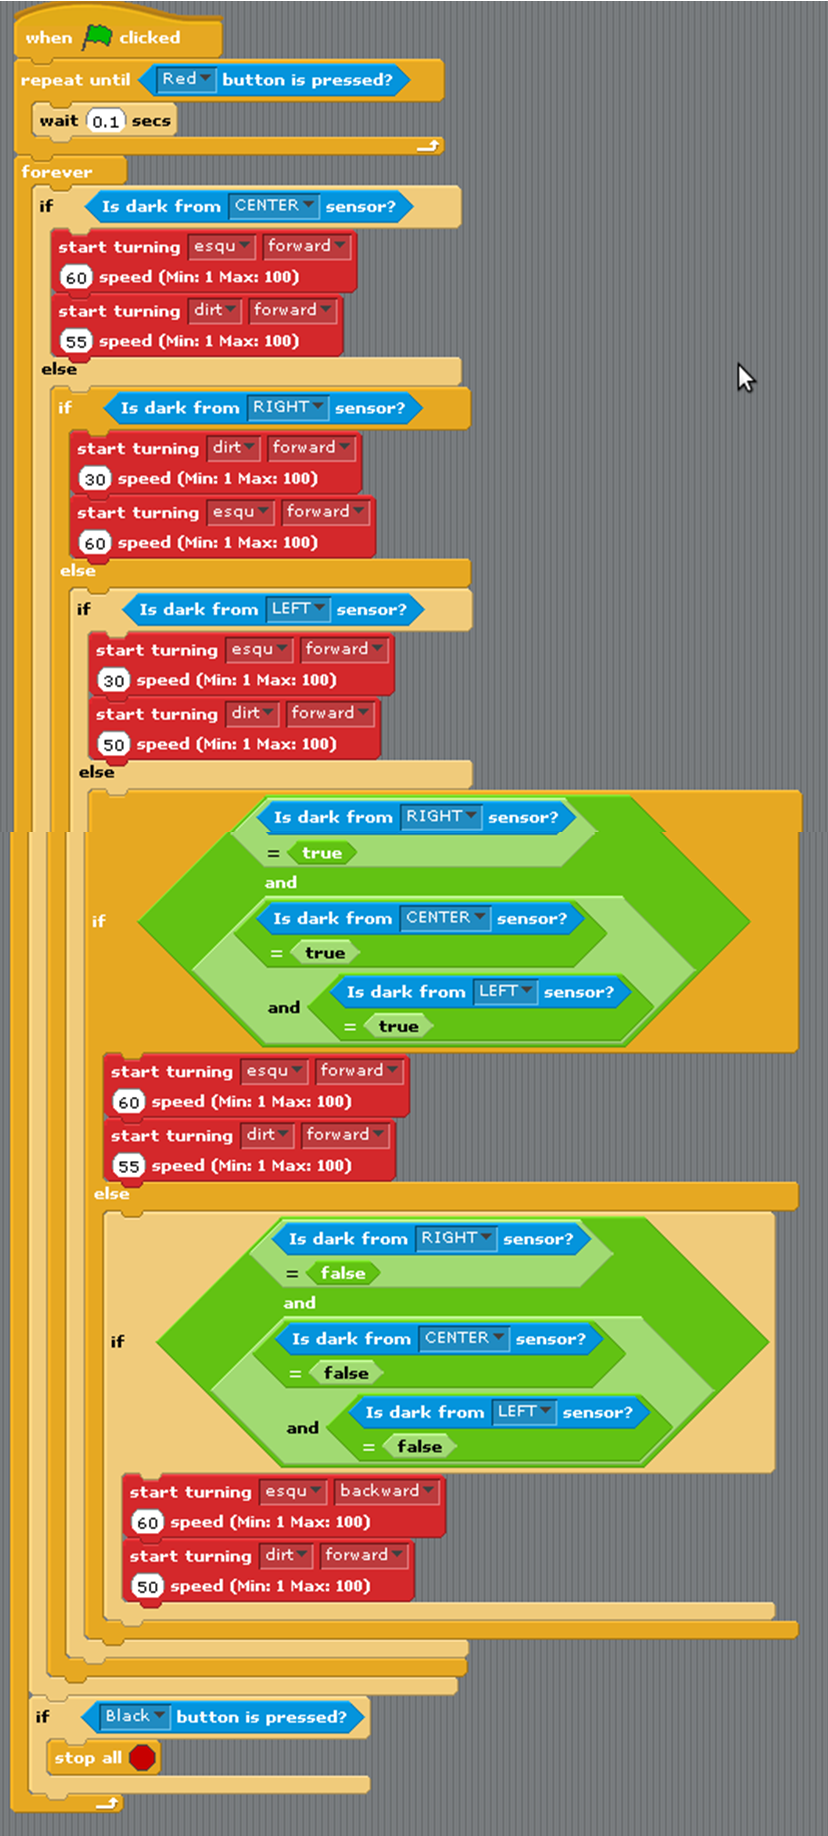
\includegraphics[width=0.53\linewidth]{ex3}}
\caption{Resolução do problema 3 utilizando o sofware DETInchanting.}
\label{fig:speciation}
\end{figure}

\subsection{Problema 4}

Através da implementação, criação e posterior uploud do programa apresentado na Figura 10, conseguimos obdecer ao enunciado do Problema 4.

\begin{figure}[H]
\center{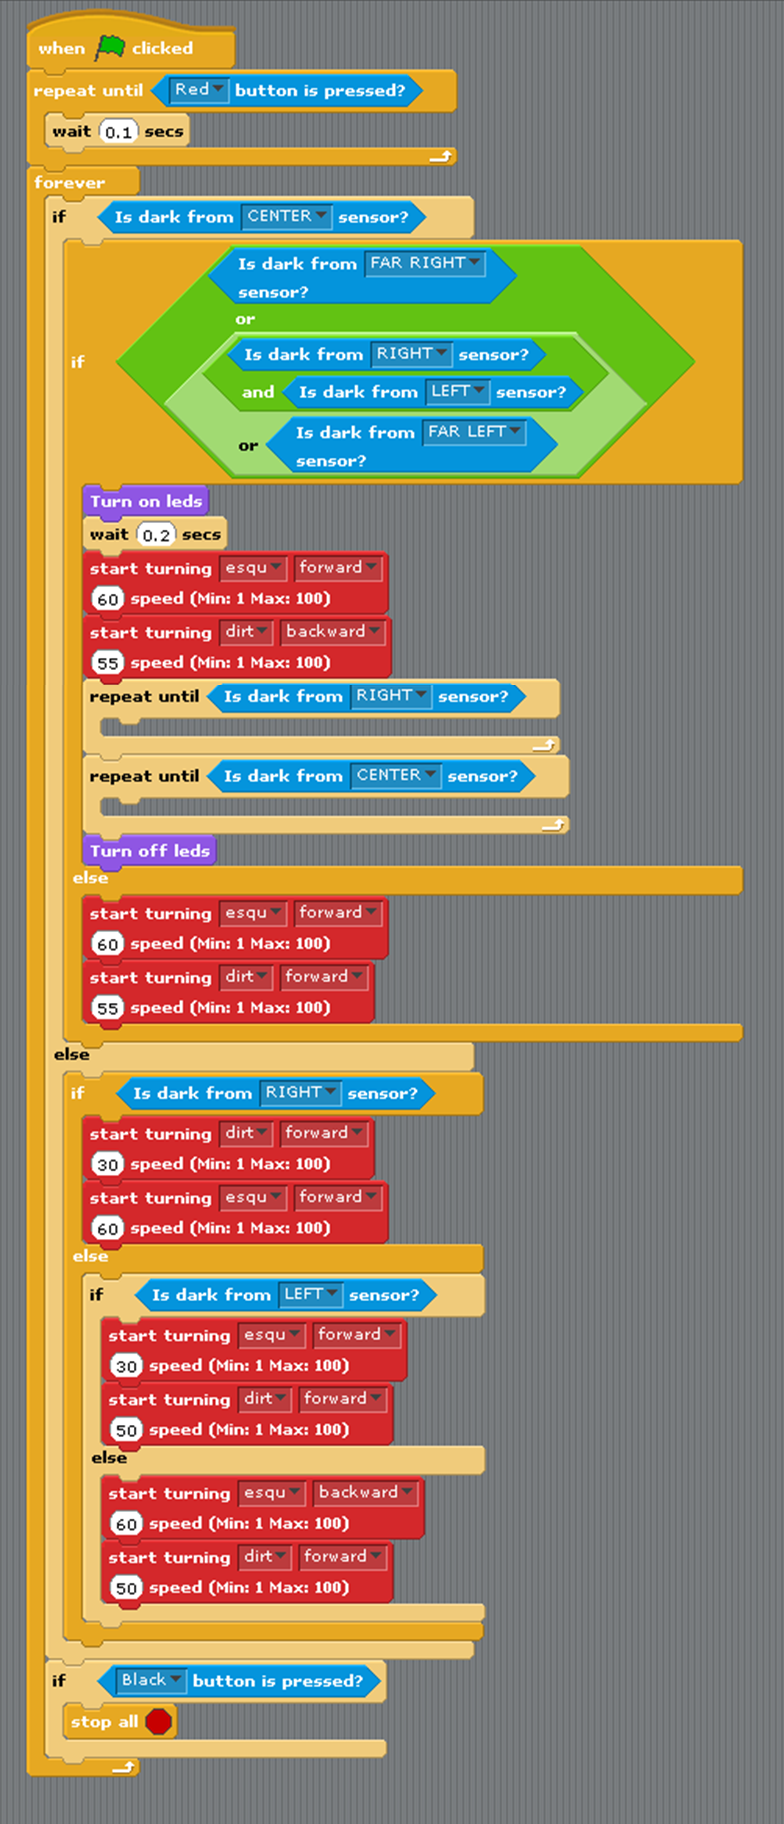
\includegraphics[width=0.5\linewidth]{ex4}}
\caption{Resolução do problema 4 utilizando o sofware DETInchanting.}
\label{fig:speciation}
\end{figure}



\subsection{Problema 5}

Devido à falta de tempo, não nos foi possível realizar e programar o Problema 5. Na próxima secção iremos apresentar um esquema que permitirá compreender o funcionamento deste programa. 



 \newpage
 






\section{Análise dos Resultados}


\subsection{Problema 1}

Através da execução do programa apresentado na secção acima, relativamente a este problema, não alcançámos grandes dificuldades no seu desenvolvimento. O nosso robô obedeceu ao esquema que se encontra representado na figura seguinte, daí pensamos que o programa estará a funcionar em perfeitas condições.

Como já dissemos anteriormente, não tivemos problemas na execução deste programa, embora inicialmente estavamos um pouco em dúvida em relação ao blocos que teriamos de utilizar.  

\begin{figure}[H]
\center{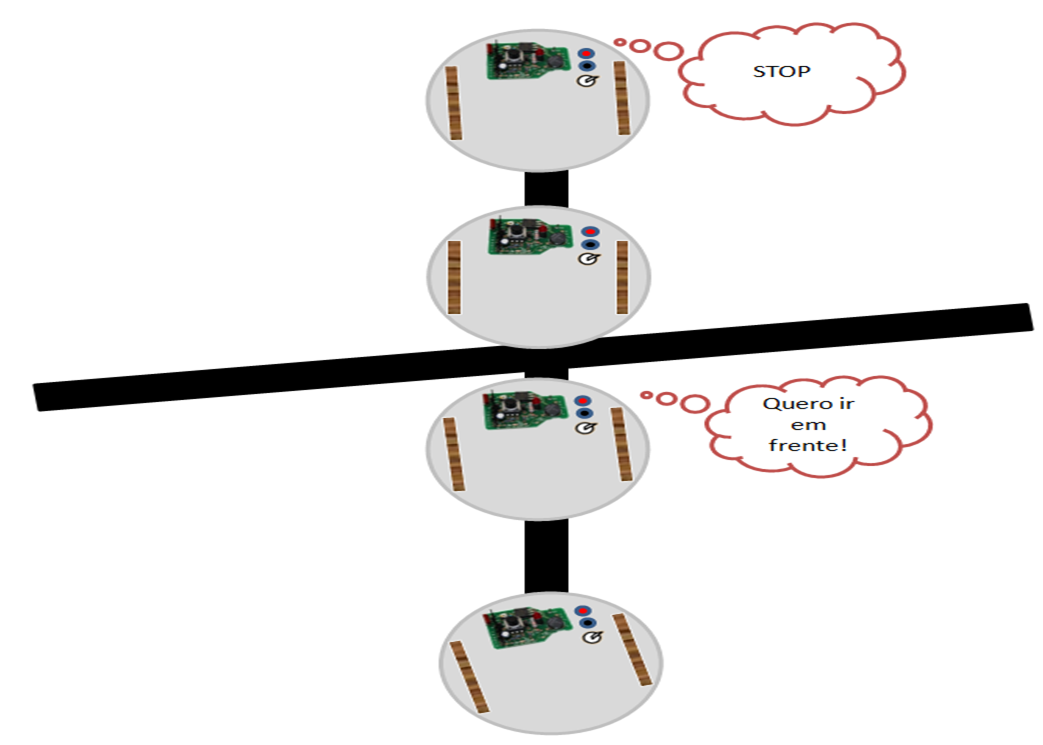
\includegraphics[width=0.8\linewidth]{esq1}}
\caption{Esquema estroboscópico do Problema 1.}
\label{fig:speciation}
\end{figure}

\newpage
\subsection{Problema 2}

Como o problema 2 resume-se a uma adaptação do problema 1, não tivemos grande dificuldade na sua programação. Apenas tivemos que alterar o programa 1 de modo que o robô pare a primeira vez que encontrar o cruzamento e durante 1 segundo ligue os 4 led's, de seguida o robô terá de percorrer a linha e no final desta, voltar para trás.  Nas restantes vezes que encontrar o cruzamento irá ignorar-lo e seguirá em frente, tal como está representado na figura abaixo.

Tal como no problema anterior não obtivemos grandes dificuldades na execução do algoritmo. Pensamos também que o programa está a funcionar em perfeitas condições. 


\begin{figure}[H]
\center{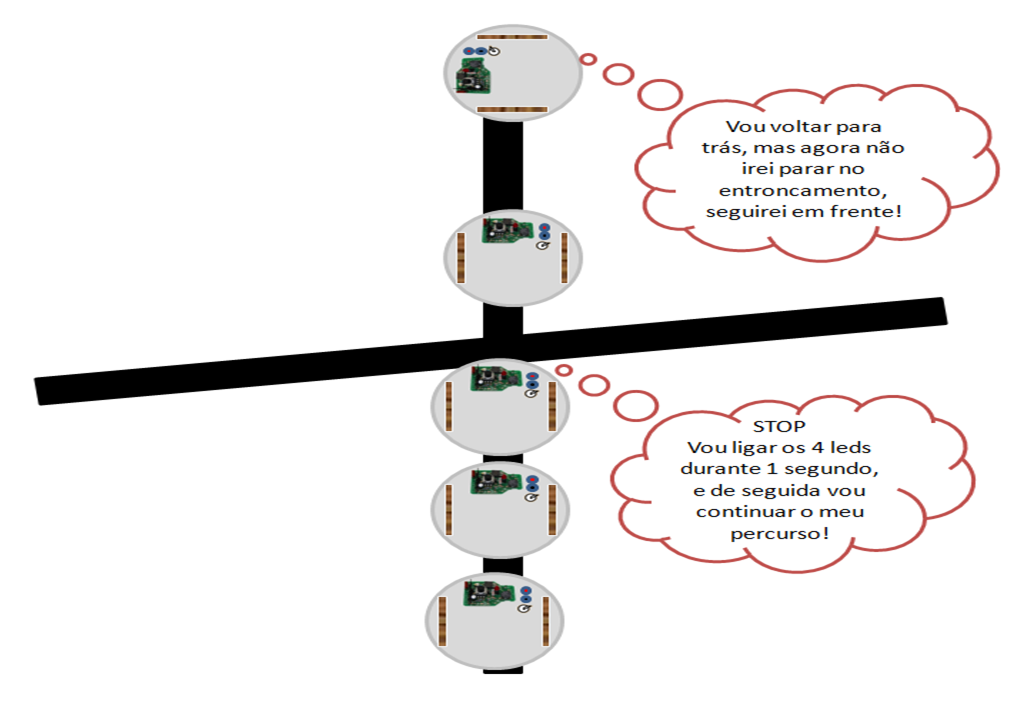
\includegraphics[width=1.0\linewidth]{esq2}}
\caption{Esquema estroboscópico do Problema 2.}
\label{fig:speciation}
\end{figure}

\newpage
\subsection{Problema 3}


Na resolução deste problema não nos deparamos com grandes dificuldades, pois como todas as situações previstas para o robô tomar decisões já tinham sido tratadas inderectamente em outros exercicios quer de outras aulas quer na própria aula em exercícios anteriores, fez com que este exercício se torna-se de certo modo mais acessivel em relação ao tempo que nos era dado. O robô conseguia sem grandes dificuldades atravessar o cruzamento sem qualquer reacção e sempre que necessário corrigia a sua posição assim como dava a volta quando chegava ao fim da linha preta.



\begin{figure}[H]
\center{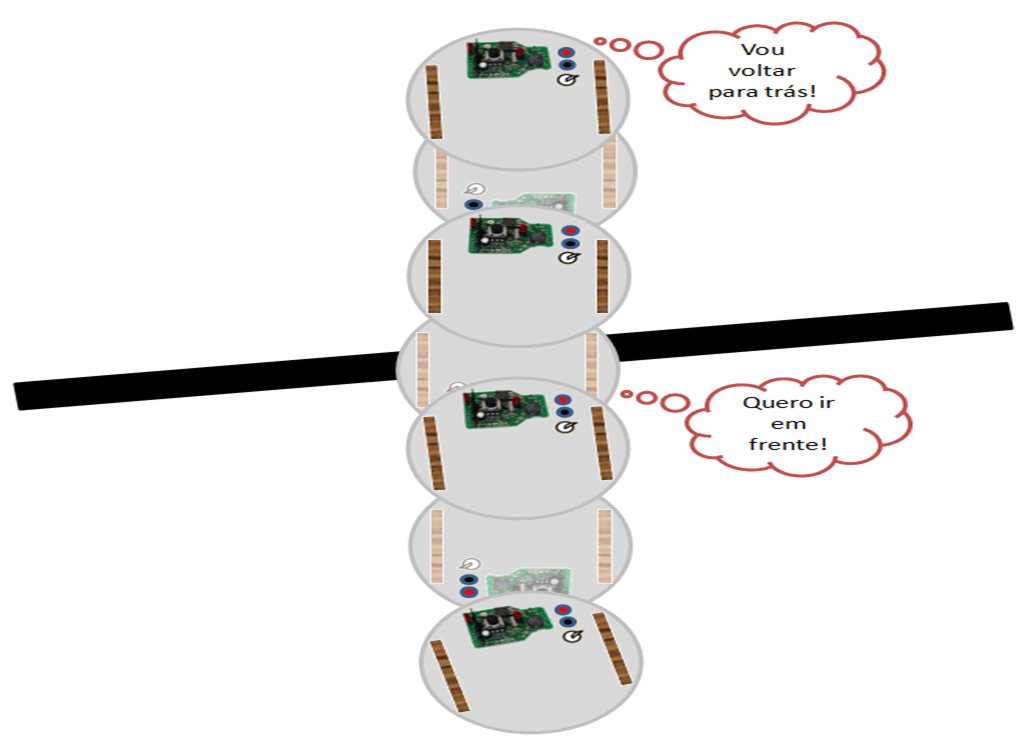
\includegraphics[width=0.9\linewidth]{esq3}}
\caption{Esquema estroboscópico do Problema 3.}
\label{fig:speciation}
\end{figure}

\newpage
\subsection{Problema 4}

A resolução deste problema foi sem dúvida a que nos causou mais problema a nivel de execução, pois não estavamos a conseguir visualizar o algoritmo que fazia o robô virar no cruzamento, fazendo com isto o robô em muitas das nossas tentativas seguir em frente, tal como se encontra representado na figura abaixo. Depois de muitas tentativas conseguimos descobrir o algoritmo certo onde depois foi preciso apenas corrigir posições após a viragem à direita assim como a própria viragem uma vez que também nos deparamos com o problema de o robô após virar não conseguir encontrar a linha preta. Foi sem dúvida o programa que nos consomiu mais tempo e uma das principais razões pelo que não tivemos tempo para resolver o problema 5. Mas no fim consideramos este problema um sucesso uma vez que o robô conseguio executar o programa na perfeição fazendo exactamente o que o enunciado pedia.


\begin{figure}[H]
\center{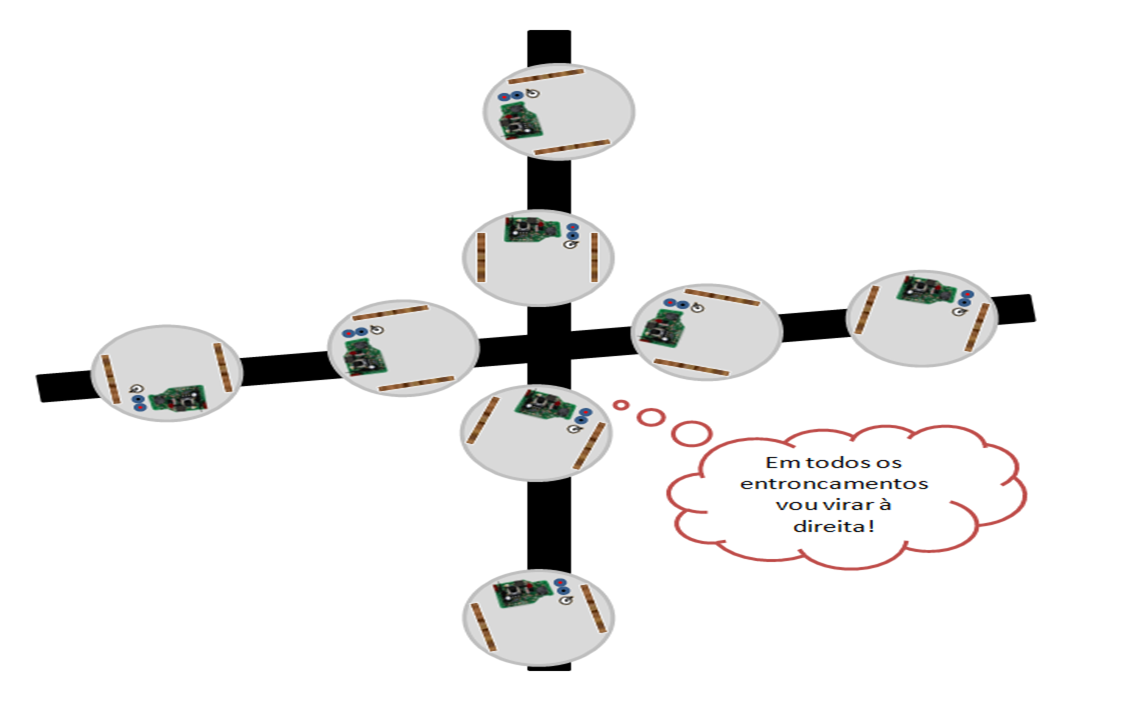
\includegraphics[width=0.9\linewidth]{esq4}}
\caption{Esquema estroboscópico do Problema 4.}
\label{fig:speciation}
\end{figure}

\newpage

\subsection{Problema 5}


Apesar de não termos tido oportunidade de resolver o programa relativo ao problema 5, devido à falta de tempo como anteriormente frisámos, deixamos aqui o esquema estrobocópico do percurso do robô respeitando o enunciado do problema.  


\begin{figure}[H]
\center{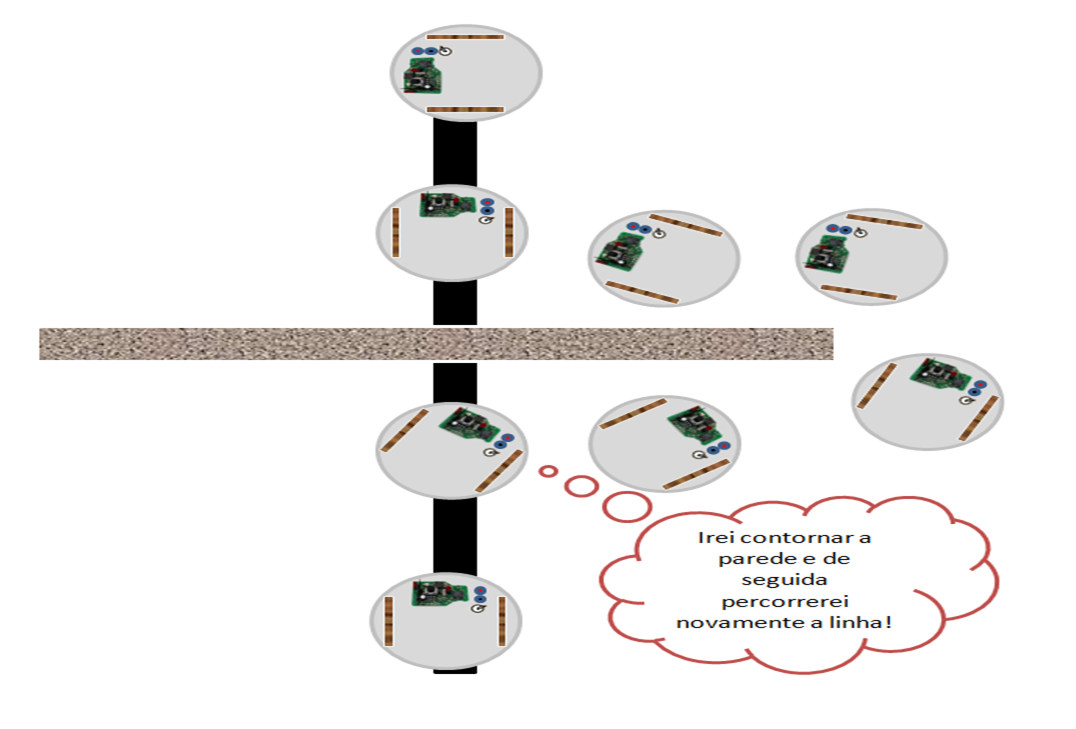
\includegraphics[width=0.9\linewidth]{esq5}}
\caption{Esquema estroboscópico do Problema 5.}
\label{fig:speciation}
\end{figure}




 \newpage

\section{Conclusões}

Chegado ao final deste relatório, é nossa intenção efetuar uma retrospetiva da evolução do mesmo, tendo em conta os problemas que nos deparámos, objetivos, e principais metodologias utilizadas.

Apesar de não termos consigo testar e programar apenas um dos problemas apresentamos, devido ao fator tempo, pensamos que os restantes foram bem conseguidos, embora com algumas dificuldades. Em todos os programas tivemos algumas duvidas na escolha dos blocos a utilizar, embora no final da aula conseguimos executar quase a totalidade dos problemas enunciados com sucesso. 








\begin{thebibliography}{99} 

\bibitem[1]{Figueredo:2009dg}
A.V.C.M. Zúquete , Site da Unidade Curicular - Introdução à Engenharia de Computadores e Telemática (12 Dezembro 2012).
\newblock Diapositivos: robô DETI PIC [Online]
\newblock {\em Available: } http://www.ieeta.pt/~avz/Aulas/IECT/12-13/docs/6-robo.pdf 

\bibitem[2]{Figueredo:2009dg}
J. Barraca, D. Gomes, A. Zúquete , Site da Unidade Curicular - Introdução à  Engenharia de Computadores e Telemática (12 Dezembro 2012).
\newblock Guião da aula prática 9 [Online]
\newblock {\em Available: } http://www.ieeta.pt/~avz/Aulas/IECT/12-13/docs/guiao-9.pdf 

 
\end{thebibliography}


\end{document}
